\section{Atomgitter}

\subsection{Modifikationen des Kohlenstoffs}
Graphit: wabenförmige Schichten aus $C_6$-Ringen $\Rightarrow$ jedes Atom geht 3 Bindungen an, das 4. Valenz-$e^-$ ist delokalisiert. Zwischen den schichten herrschen VdW-Kräfte ($\Rightarrow$ weich). Eigenschaften: sehr weich, el. Leiter, metallischer Glanz.

\subsection{Diamantartige Stoffe}
Stoffe, die sehr hart sind, Bsp. Diamant $C_D$ (Mohs-Härte 10), Quarz $SiO_2$ (7), Korund $Al_2O_3$ (9) \\

Atomarer Aufbau sehr unterschiedlich. Diamant: Atomgitter mit kovalenten Bindungen, Quarz: Atomgitter mit kovalent-ionischen Bindungen, Korund: Ionengitter (d.h. ein Salz).

\newpage

\subsection{Quarz ($SiO_2$)}
Si-Atome tetraedrisch, kovalent mit O-Atomen gebunden $\Rightarrow$ kovalent-ionische Bindungen. Aufbau ähnlich wie bei $C_D$. \\

Eigenschaften: el. Isolator, Härte 7, Schwingung bei Anlegen eines el.-mag. Feldes. \\

\subsection{Silikate}
Bsp. natürliche: Sand, Sandstein, Granit, Glimmer, Smaragd, Asbest; synthetische: Glas, Zement, Beton, Glaskeramik \\

\subsubsection{Atomarer Aufbau}
Aus $SiO_4^{x-}$ Tetraedern aufgebaut. \\

\begin{figure}[htbp]
	\centering
	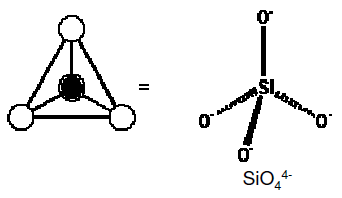
\includegraphics[width=0.4\linewidth]{images/8_SiO4.png}
\end{figure}

Unterschiedliche Verknüpfungen der Tetraeder ergeben verschiedene Silikate. Bsp. Gruppensilikat $Si_2O_7^{6-}$ (zwei Tetraeder), Ringsilikate (unterschiedlich grosse Ringe möglich), Kettensilikate, Bandsilikate  (siehe Bild unten), Schichtsilikate (Bandsilikate nebeneinander angeordnet)

\begin{figure}[htbp]
	\centering
	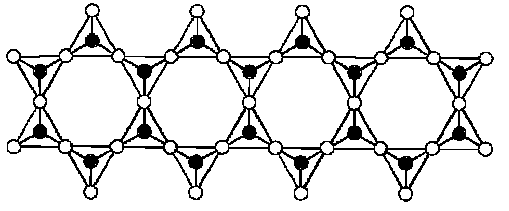
\includegraphics[width=0.7\linewidth]{images/8_Bandsilikat.png}
\end{figure}

3-dimensionales Atomgitter (Gerüstsilikat) $\Rightarrow$ $SiO_2$ Quarz

\subsubsection{Salzartige Silikate}
Nicht verknüpfte O-Atome sind an H oder $M^{a+}$ Kationen gebunden. Viele Minerale sind salzartige Stoffe mit Silikat-Anionen, z.B. Olivin, Aquamarin, Smaragd, Tonminerale (Ton, Talk), Glimmer. \\

Tonminerale sind sehr weich, leicht spaltbar und haben ein gutes Quellvermögen, weil diese aus durch VdW-Kräften zusammengehaltenen Silikatschichten bestehen. Entlang dieser Spalten sind die Tonminerale gut spaltbar oder es können Teilchen eingelagert werden. 

\subsection{Glas}
Gläser sind amorphe Stoffe. Bsp. Quarzglas: amorphes $SiO_2$ mit verzerrten Tetraedern.